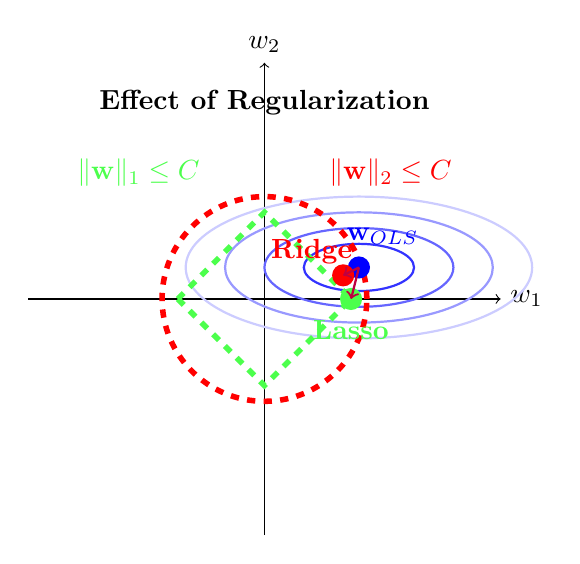
\begin{tikzpicture}[scale=1.0]
  \draw[->] (-3,0) -- (3,0) node[right] {$w_1$};
  \draw[->] (0,-3) -- (0,3) node[above] {$w_2$};
  
  % Loss contours (more elongated to show effect better)
  \draw[thick, blue!20] (1.2,0.4) ellipse (2.2 and 0.9);
  \draw[thick, blue!40] (1.2,0.4) ellipse (1.7 and 0.7);
  \draw[thick, blue!60] (1.2,0.4) ellipse (1.2 and 0.5);
  \draw[thick, blue!80] (1.2,0.4) ellipse (0.7 and 0.3);
  
  % L2 constraint (circle) - more prominent
  \draw[thick, red, dashed, line width=2pt] (0,0) circle (1.3);
  \node[red] at (1.6, 1.6) {$\|\mathbf{w}\|_2 \leq C$};
  
  % L1 constraint (diamond) - more prominent
  \draw[thick, green!70, dashed, line width=2pt] (-1.1,0) -- (0,1.1) -- (1.1,0) -- (0,-1.1) -- cycle;
  \node[green!70] at (-1.6, 1.6) {$\|\mathbf{w}\|_1 \leq C$};
  
  % Points - larger and more prominent
  \fill[blue] (1.2, 0.4) circle (4pt);
  \node[blue] at (1.5, 0.8) {$\mathbf{w}_{\text{OLS}}$};
  
  \fill[red] (1.0, 0.3) circle (4pt);
  \node[red] at (0.6, 0.6) {\textbf{Ridge}};
  
  \fill[green!70] (1.1, 0) circle (4pt);
  \node[green!70] at (1.1, -0.4) {\textbf{Lasso}};
  
  % Title
  \node at (0, 2.5) {\textbf{Effect of Regularization}};
  
  % Arrows showing the effect
  \draw[purple, thick, ->] (1.2, 0.4) -- (1.0, 0.3);
  \draw[purple, thick, ->] (1.2, 0.4) -- (1.1, 0);
\end{tikzpicture}
